% ============================================================
% Rapport Technique --- Rapport 4
% An Agentic Framework for IaC Misconfiguration Analysis
% and Remediation
%
% Ahmedou Yahye Kheyri
% Supervised by: Hala Bezine
% Faculté des Sciences de Sfax --- Master MRSI
% 2025--2026
% ============================================================

\documentclass[12pt, a4paper]{report}

% ---- Encoding & Language ----
\usepackage[utf8]{inputenc}
\usepackage[T1]{fontenc}
\usepackage[english]{babel}

% ---- Layout ----
\usepackage[
  top=2.5cm, bottom=2.5cm,
  left=3cm,  right=2.5cm
]{geometry}
\usepackage{setspace}
\onehalfspacing
\setlength{\parindent}{1.2em}
\setlength{\parskip}{0.4em}
\setlength{\headheight}{14pt}

% ---- Fonts ----
\usepackage{lmodern}
\usepackage{microtype}

% ---- Math ----
\usepackage{amsmath}
\usepackage{amssymb}
\usepackage{pifont}
\newcommand{\cmark}{\ding{51}}
\newcommand{\xmark}{\ding{55}}

% ---- Graphics & Tables ----
\usepackage{graphicx}
\usepackage{float}
\usepackage{booktabs}
\usepackage{tabularx}
\usepackage{multirow}
\usepackage{longtable}
\usepackage{array}
\usepackage[table,xcdraw]{xcolor}

% ---- Code Listings ----
\usepackage{listings}
\usepackage{lstautogobble}

\definecolor{codegreen}{rgb}{0.0,0.5,0.0}
\definecolor{codegray}{rgb}{0.5,0.5,0.5}
\definecolor{codepurple}{rgb}{0.58,0,0.82}
\definecolor{backcolour}{rgb}{0.97,0.97,0.97}
\definecolor{codeblue}{rgb}{0.0,0.0,0.7}

\lstdefinestyle{iacstyle}{
  backgroundcolor=\color{backcolour},
  commentstyle=\color{codegreen}\itshape,
  keywordstyle=\color{codeblue}\bfseries,
  stringstyle=\color{codepurple},
  basicstyle=\ttfamily\small,
  breakatwhitespace=false,
  breaklines=true,
  captionpos=b,
  keepspaces=true,
  numbers=left,
  numbersep=6pt,
  numberstyle=\tiny\color{codegray},
  showspaces=false,
  showstringspaces=false,
  showtabs=false,
  tabsize=2,
  frame=single,
  rulecolor=\color{gray!40},
  autogobble=true
}
\lstset{style=iacstyle}

% ---- TikZ ----
\usepackage{tikz}
\usetikzlibrary{shapes.geometric, arrows.meta, positioning, fit, backgrounds, calc}

% ---- PGFPlots ----
\usepackage{pgfplots}
\pgfplotsset{compat=1.18}
\usepackage{pgfplotstable}

% ---- Colors ----
\definecolor{agentblue}{RGB}{70,130,180}
\definecolor{analyzergreen}{RGB}{60,160,90}
\definecolor{kbpurple}{RGB}{130,80,170}
\definecolor{generatororange}{RGB}{210,120,30}
\definecolor{validatorsalmon}{RGB}{200,80,60}
\definecolor{formatterpink}{RGB}{180,60,120}
\definecolor{lightgray}{RGB}{245,245,245}
\definecolor{critblue}{RGB}{40,70,140}
\definecolor{critred}{RGB}{180,40,40}
\definecolor{critgreen}{RGB}{40,140,70}
\definecolor{critorange}{RGB}{200,110,30}

% ---- Headers & Footers ----
\usepackage{fancyhdr}
\pagestyle{fancy}
\fancyhf{}
\fancyhead[L]{\small\leftmark}
\fancyhead[R]{\small\thepage}
\fancyfoot[C]{\small Rapport~4 --- Ahmedou Yahye Kheyri --- Faculté des Sciences de Sfax}
\renewcommand{\headrulewidth}{0.4pt}
\renewcommand{\footrulewidth}{0.2pt}

% ---- Hyperlinks ----
\usepackage[
  colorlinks=true,
  linkcolor=blue!70!black,
  citecolor=blue!60!black,
  urlcolor=blue!80!black,
  bookmarks=true,
  bookmarksnumbered=true
]{hyperref}
\usepackage{url}

% ---- Bibliography ----
\usepackage[numbers,sort&compress]{natbib}
\bibliographystyle{IEEEtranN}

% ---- Caption ----
\usepackage[font=small,labelfont=bf]{caption}
\usepackage{subcaption}

% ---- Boxes ----
\usepackage{tcolorbox}
\tcbuselibrary{breakable, skins}

\newtcolorbox{researchbox}[1][]{
  colback=blue!5!white, colframe=blue!50!black,
  fonttitle=\bfseries, title={#1},
  breakable, enhanced
}

\newtcolorbox{definitionbox}[1][]{
  colback=green!5!white, colframe=green!50!black,
  fonttitle=\bfseries, title={#1},
  breakable, enhanced
}

\newtcolorbox{findingbox}[1][]{
  colback=yellow!8!white, colframe=orange!55!black,
  fonttitle=\bfseries, title={#1},
  breakable, enhanced
}

\newtcolorbox{warningbox}[1][]{
  colback=red!5!white, colframe=red!55!black,
  fonttitle=\bfseries, title={#1},
  breakable, enhanced
}

% ---- Chapter style ----
\usepackage{titlesec}
\titleformat{\chapter}[display]
  {\normalfont\huge\bfseries\color{agentblue}}
  {\chaptertitlename\ \thechapter}{16pt}{\Huge}
\titlespacing*{\chapter}{0pt}{-10pt}{20pt}

% ---- Acronyms ----
\usepackage[acronym,toc]{glossaries}
\makeglossaries
\newacronym{iac}{IaC}{Infrastructure as Code}
\newacronym{llm}{LLM}{Large Language Model}
\newacronym{rag}{RAG}{Retrieval-Augmented Generation}
\newacronym{crag}{CRAG}{Corrective Retrieval-Augmented Generation}
\newacronym{cwe}{CWE}{Common Weakness Enumeration}
\newacronym{nlp}{NLP}{Natural Language Processing}
\newacronym{tp}{TP}{True Positive}
\newacronym{fp}{FP}{False Positive}
\newacronym{fn}{FN}{False Negative}
\newacronym{pvr}{PVR}{Patch Validity Rate}
\newacronym{ser}{SER}{Smell Elimination Rate}
\newacronym{nnir}{NNIR}{No-New-Issues Rate}
\newacronym{api}{API}{Application Programming Interface}
\newacronym{kics}{KICS}{Keeping Infrastructure as Code Secure}
\newacronym{cfn}{CFN}{AWS CloudFormation}
\newacronym{cdk}{CDK}{Cloud Development Kit}
\newacronym{ast}{AST}{Abstract Syntax Tree}
\newacronym{sota}{SOTA}{State of the Art}
\newacronym{cve}{CVE}{Common Vulnerabilities and Exposures}

% ============================================================
\begin{document}
% ============================================================

% ---- Title Page ----
\begin{titlepage}
  \centering

  \vspace*{2.5cm}
  {\small Ministère de l'Enseignement Supérieur, de la Recherche Scientifique
   et de la Technologie}\\[4pt]
  {\small Université de Sfax \enspace\textbar\enspace Faculté des Sciences de Sfax}\\[4pt]
  {\small Département d'Informatique \enspace\textbar\enspace Master MRSI}

  \vspace{2.5cm}

  \noindent\rule{\linewidth}{0.6pt}\\[0.8cm]

  {\Large\bfseries\color{agentblue}
    An Agentic Framework for Infrastructure as Code\\[6pt]
    Misconfiguration Analysis and Remediation
  }\\[0.8cm]

  \noindent\rule{\linewidth}{0.6pt}

  \vspace{0.6cm}
  {\normalsize\itshape Technical Report --- Rapport 4}\\[3pt]
  {\small Technology Positioning, Empirical Plan, and Repositioned Contributions}

  \vspace{2.5cm}
  \begin{minipage}[t]{0.45\textwidth}
    \raggedright
    {\small\bfseries Prepared by}\\[4pt]
    {\normalsize Ahmedou Yahye Kheyri}
  \end{minipage}
  \hfill
  \begin{minipage}[t]{0.45\textwidth}
    \raggedleft
    {\small\bfseries Supervised by}\\[4pt]
    {\normalsize Pr.\ Hala Bezine}
  \end{minipage}

  \vfill
  {\small\textit{Keywords:}\enspace
   Agentic Framework \textbullet\
   Infrastructure as Code \textbullet\
   Security Smells \textbullet\
   Retrieval-Augmented Generation \textbullet\
   Patch Validation \textbullet\
   Large Language Models}\\[1.2cm]

  {\small Academic Year 2025--2026 \enspace\textbar\enspace April 2026}
  \vspace{1cm}

\end{titlepage}

% ---- Abstract ----
\chapter*{Abstract}
\addcontentsline{toc}{chapter}{Abstract}

This fourth technical report consolidates the design (Rapport~2), the corpus
(Rapport~3), and the internal critique (Rapport-Critique) of the thesis into
a single coherent positioning of the work as of April~2026. Two changes
relative to Rapport~2 are central. First, the project is repositioned around
the empirical contribution that has actually materialised: a
$33{,}667$-record \gls{iac} security fix corpus, scraped, classified by a
44-entry smell taxonomy, and undergoing dynamic validation by
Checkov~\citep{checkov2024}. Second, the contribution is reframed from a
generic ``agentic framework for IaC security'' into a specifically positioned
artefact within a 2025--2026 benchmark landscape: \emph{agentic IaC
remediation with independent scanner-based validation}. A landscape grid is
constructed across PatchEval~\citep{lyu2024patcheval},
AutoPatchBench~\citep{autopatchbench2025}, SEC-bench~\citep{secbench2025},
SecRepoBench~\citep{secrepobench2025}, IaC-Eval~\citep{kon2024iaceval},
Multi-IaC-Eval~\citep{multi2025iaceval}, IntelliSA~\citep{intellisa2026},
SecLLM~\citep{devito2025secllm}, and GenSIAC~\citep{li2025gensiac}, and the
target cell is shown to be unoccupied. The framework architecture is carried
over from Rapport~2 with two amendments: KICS~\citep{kics2024} is added as a
second validator to extend coverage to Ansible, Kubernetes, Dockerfile, and
CloudFormation, and the log-prob-based confidence score is replaced by a
self-consistency surrogate. The evaluation methodology is reduced from the
previously claimed eighteen metrics to a defensible eight, with \gls{pvr},
\gls{ser}, and \gls{nnir} retained as the primary outcomes and the Wilcoxon
rank-sum analysis kept as the inferential test. A planned experimental
protocol is given for Configurations~B, C, and~D on a stratified $3{,}371$-record
held-out test split, with IntelliSA~\citep{intellisa2026} fixed as the
detection-side \gls{sota} baseline. Threats to validity are stated explicitly
and an updated implementation timeline is given.

\bigskip
\noindent\textbf{Keywords:} Agentic Framework, Infrastructure as Code,
Security Smells, Retrieval-Augmented Generation, Patch Validation, Large
Language Models, Empirical Software Engineering.

% ---- TOC ----
\tableofcontents
\listoffigures
\listoftables

\printglossary[type=\acronymtype, title=List of Acronyms]

% ============================================================
\chapter{Technology Timeline and Positioning}
\label{chap:timeline}
% ============================================================

\section{Why this chapter exists}

Rapport~2 introduced the framework on the strength of three references whose
most recent publication was 2024 and whose detection baseline was an
\gls{llm}-only system (SecLLM, GenSIAC, War et al.). Between writing
Rapport~2 and writing this report, the relevant literature has moved: a new
\gls{sota} on \gls{iac} smell detection (IntelliSA, January~2026), a
patch-validation benchmark with the same dynamic-validation philosophy as
this thesis (PatchEval, November~2025), and a multi-format \gls{iac}
mutation benchmark (Multi-IaC-Eval, September~2025) have all appeared.
A repositioning is therefore required \emph{before} reporting any further
experiments.

This chapter rebuilds the temporal context, then collapses it into a
two-dimensional landscape grid (task $\times$ domain) that locates the thesis
contribution precisely.

\section{Technology evolution, 2019--2026}

\begin{figure}[H]
  \centering
  \resizebox{\linewidth}{!}{%
  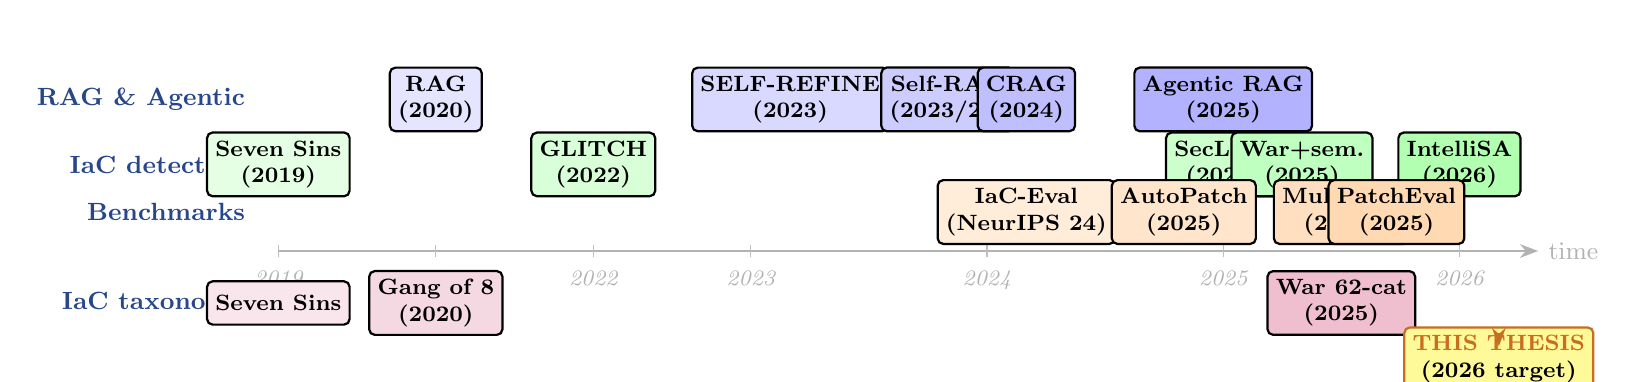
\begin{tikzpicture}[
    yscale=0.55,
    node distance=0.2cm,
    milestone/.style={
      draw, thick, rounded corners=2pt,
      inner sep=3pt, font=\footnotesize\bfseries,
      align=center, minimum height=0.55cm
    },
    track/.style={font=\small\bfseries, anchor=east, text=critblue},
    year/.style={font=\footnotesize\itshape, text=gray!60}
  ]
    \draw[-{Stealth[scale=1.0]}, thick, gray!60]
      (0,0) -- (16,0) node[right, font=\small] {time};

    \foreach \x/\year in {0/2019, 2/2020, 4/2022, 6/2023, 9/2024, 12/2025, 15/2026} {
      \draw[gray!50] (\x, -0.15) -- (\x, 0.15);
      \node[year, below=0.05cm] at (\x, -0.15) {\year};
    }

    \node[track] at (-0.3, 3.5) {RAG \& Agentic};
    \node[track] at (-0.3, 2.0) {IaC detection};
    \node[track] at (-0.3, 0.9) {Benchmarks};
    \node[track] at (-0.3, -1.2) {IaC taxonomy};

    \node[milestone, fill=blue!10] at (2, 3.5) {RAG\\(2020)};
    \node[milestone, fill=blue!15] at (6.5, 3.5) {SELF-REFINE\\(2023)};
    \node[milestone, fill=blue!20] at (8.5, 3.5) {Self-RAG\\(2023/24)};
    \node[milestone, fill=blue!25] at (9.5, 3.5) {CRAG\\(2024)};
    \node[milestone, fill=blue!30] at (12, 3.5) {Agentic RAG\\(2025)};

    \node[milestone, fill=green!10] at (0, 2.0) {Seven Sins\\(2019)};
    \node[milestone, fill=green!15] at (4, 2.0) {GLITCH\\(2022)};
    \node[milestone, fill=green!20] at (12, 2.0) {SecLLM\\(2025)};
    \node[milestone, fill=green!25] at (13, 2.0) {War+sem.\\(2025)};
    \node[milestone, fill=green!30] at (15, 2.0) {IntelliSA\\(2026)};

    \node[milestone, fill=orange!15] at (9.5, 0.9) {IaC-Eval\\(NeurIPS 24)};
    \node[milestone, fill=orange!20] at (11.5, 0.9) {AutoPatch\\(2025)};
    \node[milestone, fill=orange!25] at (13.5, 0.9) {Multi-IaC\\(2025)};
    \node[milestone, fill=orange!30] at (14.2, 0.9) {PatchEval\\(2025)};

    \node[milestone, fill=purple!10] at (0, -1.2) {Seven Sins};
    \node[milestone, fill=purple!15] at (2, -1.2) {Gang of 8\\(2020)};
    \node[milestone, fill=purple!25] at (13.5, -1.2) {War 62-cat\\(2025)};

    \node[milestone, fill=yellow!40, draw=critorange, thick] at (15.5, -2.5)
      {\bfseries\color{critorange} THIS THESIS\\(2026 target)};
    \draw[-{Stealth[scale=1.0]}, thick, critorange]
      (15.5, -1.9) -- (15.5, -2.2);
  \end{tikzpicture}
  }
  \caption{Technology-evolution timeline across four tracks: agentic
    \gls{rag}, \gls{iac} smell detection, benchmarks, and \gls{iac}
    taxonomies. The thesis target sits at the intersection of all four:
    a remediation contribution that uses the 2024-era \gls{crag} retry
    pattern, the 2025 War 62-category taxonomy, and the
    2025 PatchEval-style scanner-validated evaluation, applied to the
    \gls{iac} domain where IntelliSA~\citep{intellisa2026} now sets the
    2026 detection baseline.}
  \label{fig:timeline}
\end{figure}

The full milestone list is given in Table~\ref{tab:timeline}. Three
observations are worth making explicit. First, the agentic \gls{rag} track
(blue) had stabilised by 2024 with \gls{crag}~\citep{yao2024crag}; everything
in 2025 builds on that pattern rather than replacing it, which justifies
keeping the framework architecture of Rapport~2 substantially intact.
Second, the \gls{iac} detection track (green) accelerated sharply in 2025;
IntelliSA~\citep{intellisa2026} (January~2026) now reports F1 between 0.77
and 0.88 with Claude-4, GPT-5, and Grok-4, redefining what counts as a
competitive detection number. Third, the benchmark track (orange) shifted
in 2025 from generation benchmarks (IaC-Eval) to validation benchmarks
(PatchEval, AutoPatchBench). This is the same shift the thesis is making.

\begin{table}[H]
  \centering
  \caption{Milestone list backing Figure~\ref{fig:timeline}.}
  \label{tab:timeline}
  \small
  \begin{tabularx}{\linewidth}{lll X}
    \toprule
    \textbf{Year} & \textbf{Track} & \textbf{Milestone} & \textbf{Relevance to thesis} \\
    \midrule
    2019 & Taxonomy & Rahman ``Seven Sins''~\citep{rahman2019seven} & Foundational smell vocabulary; basis of the 44-entry classifier of Rapport~3 \\
    2020 & RAG & Lewis et al. (NeurIPS) & First Naive RAG paper; baseline of the retriever family used here \\
    2020 & Taxonomy & Rahman ``Gang of Eight''~\citep{rahman2020gang} & Extended vocabulary; merged into the project taxonomy \\
    2022 & IaC static & GLITCH~\citep{saavedra2022glitch} (ASE) & Polyglot IR-based detection; one of the validators considered alongside Checkov and KICS \\
    2023 Feb & Tool-use & Toolformer~\citep{schick2023toolformer} & Foundational paper for tool-augmented \glspl{llm}; informs the validator-as-tool design \\
    2023 Mar & Self-correction & SELF-REFINE~\citep{madaan2023selfrefine} & Iterative self-feedback; basis of the retry loop in the central agent \\
    2023 May & Active RAG & FLARE~\citep{jiang2023flare} & Query refinement on failure; informs the retriever's failure handling \\
    2023 Oct & Self-RAG & Asai et al.~\citep{asai2023selfrag} (ICLR 2024) & \gls{llm} decides when to retrieve; design alternative considered and rejected for budget reasons \\
    2024 Jan & CRAG & Yao et al.~\citep{yao2024crag} & Corrective \gls{rag} with retry; the chosen retriever pattern \\
    2024 Feb & RAGAS & Es et al.~\citep{es2024ragas} & Standard \gls{rag} evaluation; source of Context Recall / Context Precision metrics \\
    2024 Dec & IaC-Eval (NeurIPS) & Kon et al.~\citep{kon2024iaceval} & \gls{iac} generation benchmark; GPT-4 pass@1 = 19.4\%; not directly comparable but cited for difficulty calibration \\
    2025 Apr & AutoPatchBench & Meta~\citep{autopatchbench2025} & Tool-validated patch benchmark at industrial scale; methodological precursor to \gls{pvr} \\
    2025 Apr & SecRepoBench & \citep{secrepobench2025} & Repo-scale secure code generation; out-of-domain reference \\
    2025 May & GenSIAC & Li et al.~\citep{li2025gensiac} & Instruction-tuned \gls{llm} for \gls{iac}; F1 0.30 $\to$ 0.85; closest to the fix-generator module \\
    2025 Jun & SEC-bench & \citep{secbench2025} & Agent-built \gls{cve} benchmark; corroborates the scraping-pipeline approach of Rapport~3 \\
    2025 Jun & LLM vs.\ static & Gnieciak \& Szandala~\citep{gnieciak2025llmvsstatic} & Hybrid \gls{llm}+static approaches outperform either alone; supports the framework's hybrid design \\
    2025 Sep & Multi-IaC-Eval & \citep{multi2025iaceval} & Cross-format \gls{iac} mutation; same insecure $\to$ secure operation as this thesis, but evaluation-only, not framework \\
    2025 Sep & War semantic & \citep{war2025detection} & CodeBERT/LongFormer on \gls{iac}; P/R 0.92/0.88; one of the contextual-analyzer references \\
    2025 Oct & SecLLM (IEEE Access) & \citep{devito2025secllm} & Prompt-engineered \gls{llm} for \gls{iac} detection \\
    2025 Nov & War taxonomy update & \citep{war2025taxonomy} & 62-category \gls{iac} smell taxonomy; reduced to 44 working entries in the project classifier \\
    2025 Nov & PatchEval & \citep{lyu2024patcheval} & 1000 \glspl{cve}, 65 \glspl{cwe}, dynamic validation; closest methodological neighbour to \gls{pvr} \\
    2026 Jan & IntelliSA & \citep{intellisa2026} & Symbolic + neural hybrid; F1 0.77--0.88 with Claude-4 / GPT-5 / Grok-4; \textbf{this is the detection \gls{sota} to compare against} \\
    \midrule
    \rowcolor{yellow!15}
    \textbf{2026 Apr} & \textbf{This thesis} &
    \textbf{Agentic IaC remediation with scanner validation} &
    \textbf{The unoccupied cell of Table~\ref{tab:landscape}} \\
    \bottomrule
  \end{tabularx}
\end{table}

\section{Landscape grid: task $\times$ domain}

\begin{table}[H]
  \centering
  \caption{Benchmark landscape, April~2025 -- April~2026.}
  \label{tab:landscape}
  \small
  \begin{tabularx}{\linewidth}{l X l}
    \toprule
    \textbf{Benchmark} & \textbf{Task $\times$ Domain (key numbers)} & \textbf{Cite} \\
    \midrule
    IaC-Eval & \gls{iac} \emph{generation} $\times$ Terraform/AWS; 458 scenarios; GPT-4 pass@1 = 19.4\% & \citep{kon2024iaceval} \\
    Multi-IaC-Eval & \gls{iac} \emph{mutation} $\times$ \gls{cfn}/Terraform/\gls{cdk}; synthetic triples with \gls{llm} validation & \citep{multi2025iaceval} \\
    IntelliSA & \gls{iac} \emph{smell detection} $\times$ Puppet/Ansible/Chef; symbolic + neural; F1 0.77--0.88 & \citep{intellisa2026} \\
    SecLLM & \gls{iac} \emph{smell detection} $\times$ Ansible/Chef/Puppet; prompt-engineered GPT-4o-mini/Qwen-2.5; F1 up to 0.90 & \citep{devito2025secllm} \\
    GenSIAC & \gls{iac} \emph{secure generation} $\times$ multi-tool; instruction-tuning; F1 0.30 $\to$ 0.85 & \citep{li2025gensiac} \\
    \midrule
    PatchEval & Patch \emph{generation} $\times$ 1000 \glspl{cve} (Python/Go/JS); 65 \glspl{cwe}; dynamic sandbox + static similarity & \citep{lyu2024patcheval} \\
    AutoPatchBench & Patch \emph{generation} $\times$ fuzzing-found vulns in C/C++; Meta-internal & \citep{autopatchbench2025} \\
    SEC-bench & Agent-built \gls{cve} benchmark $\times$ multi-language; \gls{llm} agents construct the benchmark itself & \citep{secbench2025} \\
    SecRepoBench & Secure \emph{code generation} $\times$ real-world repository functions & \citep{secrepobench2025} \\
    \midrule
    \rowcolor{yellow!12}
    \textbf{This thesis (target)} &
    \textbf{Agentic \gls{iac} \emph{remediation}} $\times$
    \textbf{Terraform/Kubernetes/Ansible/Docker/\gls{cfn}}; with
    \textbf{independent scanner validation (\gls{pvr})} &
    --- \\
    \bottomrule
  \end{tabularx}
\end{table}

\begin{findingbox}[Niche identified]
The cell ``\gls{iac} $\times$ remediation $\times$ tool-validated'' is empty.
PatchEval and AutoPatchBench validate patches dynamically, but for general
code, not \gls{iac}. IntelliSA, SecLLM, GenSIAC operate on the \gls{iac}
domain, but on the detection or generation tasks rather than the
remediation-with-validation task. The thesis target is therefore both
unoccupied and clearly defined.
\end{findingbox}

\section{Implications for the rest of this report}

The repositioning has three operational consequences that are carried into
the next chapters:

\begin{enumerate}
  \item \textbf{Detection comparisons name a baseline.} Whenever the report
        states a P/R/F1 number for the contextual analyzer or the smell
        labelling layer, it must be paired with the IntelliSA F1 of
        0.77--0.88~\citep{intellisa2026} on a comparable evaluation set
        (Puppet/Ansible/Chef). This is enforced in Chapter~\ref{chap:eval}.
  \item \textbf{Remediation numbers carry the contribution.} \gls{pvr},
        \gls{ser}, and \gls{nnir} are the contribution-bearing metrics; no
        prior \gls{iac} benchmark computes them.
        Chapter~\ref{chap:eval} treats them as primary and the detection
        F1 as secondary.
  \item \textbf{Methodological lineage is cited.} \gls{pvr} is positioned
        as the \gls{iac}-domain analogue of the dynamic-validation strand of
        PatchEval~\citep{lyu2024patcheval} and
        AutoPatchBench~\citep{autopatchbench2025}, and that lineage is named
        explicitly in Chapter~\ref{chap:eval}.
\end{enumerate}

% ============================================================
\chapter{Updated State of the Art}
\label{chap:sota}
% ============================================================

This chapter incrementally updates the State of the Art of Rapport~2 with
the eight references that appeared between April~2025 and April~2026 and
that materially affect the thesis. The unchanged content of Rapport~2
(\gls{rag}, \gls{crag}, Self-RAG, FLARE, SELF-REFINE, Toolformer, RAGAS,
Rahman 2019/2020, GLITCH 2022, War 2025) is referenced rather than
re-narrated; the focus here is on what is new.

\section{New \gls{iac} detection baseline: IntelliSA}

IntelliSA~\citep{intellisa2026} (January~2026) combines symbolic analysis
with neural classifiers on Puppet, Ansible, and Chef and reports F1 between
$0.77$ and $0.88$ depending on the back-end \gls{llm} (Claude-4, GPT-5,
Grok-4). Two consequences for this thesis:

\begin{enumerate}
  \item Any detection-side number reported by the contextual analyzer or by
        the smell-labelling pipeline of Rapport~3 must be compared against
        IntelliSA on the same domain (Ansible / Chef / Puppet) and on a
        comparable held-out split. Rapport~2's macro-F1 of $0.082$ on the
        8-file suite (Configuration~A) is not in that league and is no
        longer used as a headline.
  \item The IntelliSA paper itself is a precedent for the
        ``ensemble of static + \gls{llm}'' pattern that the thesis already
        adopts; this strengthens, rather than weakens, the framework's
        design. The novelty of the thesis lies downstream of detection,
        in the remediation loop.
\end{enumerate}

\section{Methodological lineage of \gls{pvr}: PatchEval and AutoPatchBench}

PatchEval~\citep{lyu2024patcheval} (November~2025) evaluates \gls{llm}-generated
patches for $1{,}000$ real \glspl{cve} across $65$ \gls{cwe} categories using
a combination of dynamic execution in a sandbox and static patch-similarity
scoring. AutoPatchBench~\citep{autopatchbench2025} (April~2025, Meta) does
the analogous thing for fuzzing-found vulnerabilities in C/C++ at industrial
scale. Both are out-of-domain (general code, not \gls{iac}), but both
implement the same conceptual move that justifies \gls{pvr}: \emph{a patch
is only counted as successful if a tool independent of the generator confirms
it}. \gls{pvr} is therefore positioned in Chapter~\ref{chap:eval} as the
\gls{iac}-domain analogue of this dynamic-validation pattern, and PatchEval
is cited as its closest methodological precursor.

\section{Benchmark-construction precedent: SEC-bench and SecRepoBench}

SEC-bench~\citep{secbench2025} (June~2025) demonstrates that \gls{llm} agents
can construct benchmarks themselves --- the agent reads \gls{cve} reports,
identifies the affected code, and assembles reproducible test cases. The
relevance for this thesis is that the scraping pipeline of Rapport~3 (33,667
records) is a same-spirit construction effort, even though it operates at
the \gls{iac}-commit level rather than the \gls{cve} level. SEC-bench gives
the practice a published precedent.

SecRepoBench~\citep{secrepobench2025} (April~2025) extends secure-code
generation evaluation to the repository scale. It is not directly comparable
because it operates on application code and uses test suites as the oracle,
but it confirms that \emph{secure} generation is now an active benchmark
category, distinct from generic generation.

\section{IaC generation calibration: IaC-Eval and Multi-IaC-Eval}

IaC-Eval~\citep{kon2024iaceval} (NeurIPS~2024) measures
Terraform-on-AWS \emph{generation} from natural-language prompts;
GPT-4 reaches a pass@1 of $19.4\%$. The number is not directly comparable
to remediation, but it calibrates the difficulty of the broader task:
\emph{producing} correct \gls{iac} from scratch is hard for top-tier
\glspl{llm}, which makes the \emph{remediation} setting (where a syntactic
skeleton already exists) genuinely easier and worth attempting separately.

Multi-IaC-Eval~\citep{multi2025iaceval} (September~2025) builds synthetic
mutation triples (insecure $\to$ secure $\to$ broken) across \gls{cfn},
Terraform, and \gls{cdk}. It is a sibling effort to the
$33{,}667$-record corpus of Rapport~3 but uses synthetic generation rather
than real commits, and is evaluated by an \gls{llm}-as-judge rather than by
external scanners. The thesis corpus is therefore complementary, not
redundant, and a comparative analysis is added to
Chapter~\ref{chap:dataset}.

\section{Survey context: agentic \gls{rag} in 2025}

The 2025 agentic-\gls{rag} survey~\citep{agenticrag2025survey} formalises a
taxonomy of agentic \gls{rag} systems by orchestration pattern (sequential,
loop-based, planner-based, multi-agent). The framework of this thesis is a
loop-based agentic \gls{rag} system in that taxonomy, with the validator as
the failure signal. The survey citation replaces the looser appeals to
``agent design'' that appeared in Rapport~2.

\section{Carry-over of unchanged sections}

The remaining content of Rapport~2's State of the Art --- the \gls{rag}
family from naive to \gls{crag}, SELF-REFINE, FLARE, Toolformer, the Rahman
2019/2020 taxonomy, GLITCH, War et al.~2025 (semantic + 62-category
taxonomy), GenSIAC, SecLLM, RAGAS, the Wilcoxon and Holm--Bonferroni
references --- carries forward unchanged and is not re-narrated here. The
references file (\texttt{references.bib}) is the single source of truth for
all citations.

\begin{findingbox}[State of the Art --- net change]
Eight new references in twelve months. One repositions the detection
baseline (IntelliSA). Two anchor the methodological lineage of \gls{pvr}
(PatchEval, AutoPatchBench). Two corroborate the benchmark construction
work of Rapport~3 (SEC-bench, SecRepoBench). Two complement the corpus on
\gls{iac} (IaC-Eval, Multi-IaC-Eval). One updates the agentic-\gls{rag}
vocabulary (agentic-RAG survey).
\end{findingbox}

% ============================================================
\chapter{Framework Architecture (Carried Over with Two Amendments)}
\label{chap:framework}
% ============================================================

The framework is not redesigned in this report. The six-module architecture
introduced in Rapport~2 (Central Agent, Contextual Analyzer, Knowledge Base,
Knowledge Retriever, Fix Generator, External Tool Integrator, Patch
Formatter) is carried forward as the canonical reference. This chapter
states only the two amendments that the critique
(\emph{Rapport-Critique}) made necessary, and a third clarification on
input/output contracts.

\section{Reference architecture (recap)}

\begin{figure}[H]
  \centering
  \resizebox{0.95\linewidth}{!}{%
  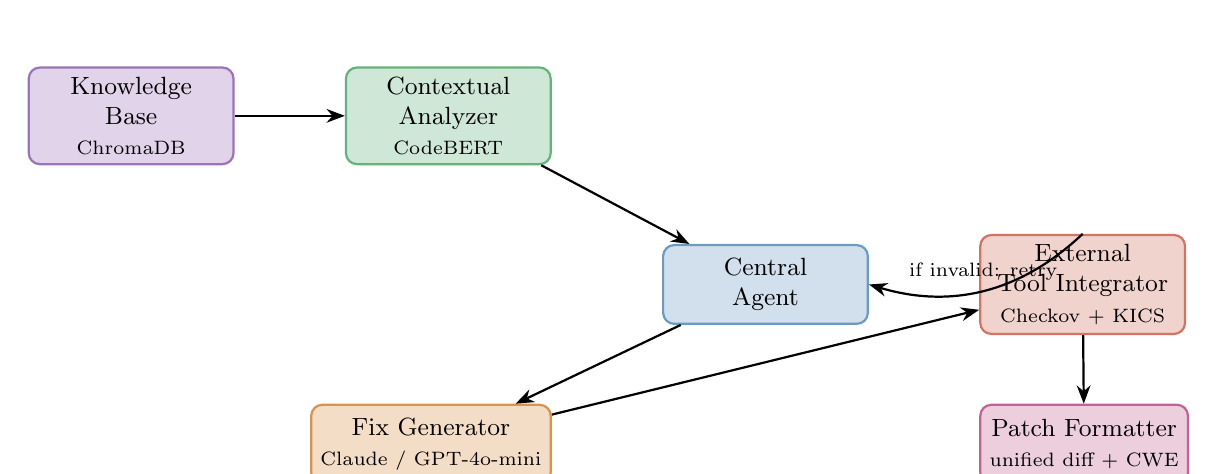
\begin{tikzpicture}[
    node distance=1.0cm and 1.4cm,
    every node/.style={font=\small},
    box/.style={
      rectangle, rounded corners=4pt, draw, thick,
      minimum width=2.6cm, minimum height=1.0cm,
      align=center, fill=lightgray
    },
    agent/.style={box, fill=agentblue!25, draw=agentblue!80, thick},
    analyzer/.style={box, fill=analyzergreen!25, draw=analyzergreen!80},
    kb/.style={box, fill=kbpurple!25, draw=kbpurple!80},
    gen/.style={box, fill=generatororange!25, draw=generatororange!80},
    val/.style={box, fill=validatorsalmon!25, draw=validatorsalmon!80},
    fmt/.style={box, fill=formatterpink!25, draw=formatterpink!80},
    arrow/.style={-{Stealth[scale=1.0]}, thick}
  ]
    \node[agent] (central) {Central\\Agent};
    \node[analyzer, above left=1.0cm and 1.4cm of central] (analyzer)
      {Contextual\\Analyzer\\\scriptsize CodeBERT};
    \node[kb, left=of analyzer] (kb) {Knowledge\\Base\\\scriptsize ChromaDB};
    \node[gen, below left=1.0cm and 1.4cm of central] (gen)
      {Fix Generator\\\scriptsize Claude / GPT-4o-mini};
    \node[val, right=of central] (val)
      {External\\Tool Integrator\\\scriptsize Checkov + KICS};
    \node[fmt, below right=1.0cm and 1.4cm of central] (fmt)
      {Patch Formatter\\\scriptsize unified diff + CWE};

    \draw[arrow] (analyzer) -- (central);
    \draw[arrow] (central) -- (gen);
    \draw[arrow] (gen) -- (val);
    \draw[arrow] (val.north) to[bend left=30] node[above, font=\scriptsize]
      {if invalid: retry} (central.east);
    \draw[arrow] (val) -- (fmt);
    \draw[arrow] (kb) -- (analyzer);
  \end{tikzpicture}
  }
  \caption{Reference architecture (carried over from Rapport~2). The two
    changes in this report are: (i)~the External Tool Integrator now runs
    KICS in addition to Checkov, and (ii)~the Fix Generator emits a
    self-consistency confidence score over $N=5$ samples instead of a
    log-prob.}
  \label{fig:arch}
\end{figure}

\section{Amendment 1: KICS as second validator}
\label{sec:kics}

\subsection{Why}

Checkov~\citep{checkov2024} is the validator chosen in Rapport~2 because it
covers Terraform comprehensively and offers a stable Python API. The
critique identified two problems:

\begin{enumerate}
  \item Checkov's coverage of Ansible, Kubernetes, Dockerfile and
        \gls{cfn} is partial; for a record whose only smell is, e.g., an
        Ansible \texttt{become: yes} pattern, Checkov produces no signal,
        and \gls{pvr} is therefore undefined for that record.
  \item Independence is the entire point of the validator. A single
        scanner produces a single source of truth; if Checkov mislabels
        a smell, the framework has no way to detect that mislabelling.
\end{enumerate}

\subsection{What changes}

KICS~\citep{kics2024} (Checkmarx) is added as a second, independent
validator. KICS covers Ansible (233 queries), \gls{cfn} (288),
Dockerfile (97), Docker Compose (43), Google Deployment Manager (38),
Azure Resource Manager (85), Crossplane (22), Kubernetes, and Terraform.
For a candidate patch, the External Tool Integrator now runs both
Checkov and KICS and produces a triple
$(s_C^{\text{before}}, s_C^{\text{after}}, s_K^{\text{before}}, s_K^{\text{after}})$
of smell sets. \gls{pvr} is then computed per scanner, and an
\emph{ensembled} \gls{pvr} is reported as an additional outcome
(definition in \S\ref{sec:metrics}).

\subsection{Where in the code}

The change is localised to
\texttt{Code/src/validator/tool\_integrator.py}; it introduces a
\texttt{KICSValidator} class with the same interface as
\texttt{CheckovValidator} and an aggregator that calls both in parallel.
The two scanners run in independent processes; the failure of either does
not block the other. Datasets for KICS positive/negative test cases live
under \texttt{datasets/kics-assets/} (sparse-checkout of the
Checkmarx/kics repository).

\section{Amendment 2: self-consistency confidence}
\label{sec:selfconsistency}

\subsection{Why}

Rapport~2 specified a confidence score derived from token log-probabilities.
The critique pointed out that the Anthropic Messages \gls{api} (the
back-end actually used in Configurations~B/C/D) does not expose token
log-probabilities. The metric is therefore not computable as written, and
any number reported under it would be either fabricated or measured on a
different model than the rest of the pipeline.

\subsection{What changes}

The confidence score is redefined as \emph{self-consistency over $N$ sampled
patches}~\citep{wang2023selfconsistency}. Concretely, for each input record
the Fix Generator is queried $N=5$ times at temperature $T=0.7$. Each of the
five candidate patches is post-processed to a normalised diff (whitespace
and comment-stripped). The confidence of the candidate that is finally
returned is the fraction of the $N$ samples that produce a diff
$\sigma$-equivalent to it, after a syntactic normalisation pass:
\begin{equation}
  \mathrm{conf}(\hat{p}) \;=\;
  \frac{1}{N}\sum_{i=1}^{N}\mathbb{1}\!\left[\mathrm{norm}(\hat{p}_i) = \mathrm{norm}(\hat{p})\right].
  \label{eq:selfconf}
\end{equation}
The metric takes values in $\{0.2, 0.4, 0.6, 0.8, 1.0\}$ for $N=5$. It is
backend-agnostic, computable on any \gls{llm}, and it correlates with patch
quality in the original self-consistency literature~\citep{wang2023selfconsistency}.

\subsection{Where in the code}

The change is localised to
\texttt{Code/src/generator/fix\_generator.py}; the
\texttt{generate\_patch()} method is wrapped to draw $N$ samples, normalise,
and aggregate. Latency cost is multiplicative in $N$; this is acknowledged
in Chapter~\ref{chap:results} as part of the runtime budget for the planned
experiments.

\section{Clarification on input/output contracts}

The framework's I/O contract is restated for completeness because Rapport~2
specified it informally. An input record is a JSON object with fields
\texttt{file\_path}, \texttt{tool} (one of \texttt{terraform}, \texttt{ansible},
\texttt{kubernetes}, \texttt{docker}, \texttt{cloudformation}),
\texttt{code\_before}, \texttt{repo}, \texttt{commit\_sha}, and
\texttt{smells\_before} (a list of taxonomy IDs). An output record adds
\texttt{code\_after\_proposed}, \texttt{diff}, \texttt{confidence} (per
Eq.~\ref{eq:selfconf}), \texttt{validator\_results} (a dict with one entry
per scanner), and \texttt{retry\_count}. The contract is stable across the
three remaining configurations of Chapter~\ref{chap:results} and is the
data shape consumed by \texttt{Code/scripts/evaluate.py}.

% ============================================================
\chapter{Dataset (33{,}667-record corpus, promoted to primary)}
\label{chap:dataset}
% ============================================================

\section{From a sanity-check suite to a primary dataset}

Rapport~2 reported preliminary results on a hand-crafted suite of 8
\gls{iac} files containing 27 manually-labelled smell instances. That suite
remains useful as an end-to-end smoke test that runs in under a minute and
that a reviewer can audit at a glance, but it is too small for any
quantitative claim about the framework. In particular, with $N\!\!=\!\!27$ and
many smell categories represented by a single instance, per-category
F1 numbers are noise.

The 33{,}667-record corpus produced by the scraping pipeline of Rapport~3
is large enough to support quantitative claims. It was constructed by
mining real Git commits (GitHub initially, GitLab planned) for paired
\emph{insecure $\to$ secure} \gls{iac} edits, classifying each diff against
a 44-entry smell taxonomy, and tiering the records by quality. This
chapter promotes that corpus to the primary evaluation dataset of the
thesis. The 8-file sanity suite is moved to an appendix and recast as a
continuous-integration unit test for the framework code.

\section{Corpus composition}

\begin{table}[H]
  \centering
  \caption{Corpus composition by \gls{iac} tool, after the salvage pass of
    Rapport~3 \S2.4. Counts may shift modestly after the Checkov
    validator finishes the full sweep (Phase~4 of
    \texttt{Code/scraping/plan.md}).}
  \label{tab:corpus}
  \small
  \begin{tabular}{lrr}
    \toprule
    \textbf{Tool} & \textbf{Records} & \textbf{Share} \\
    \midrule
    Terraform        & ~17{,}900  & 53\%  \\
    Kubernetes (YAML manifests) & ~6{,}800 & 20\% \\
    Ansible          & ~4{,}200   & 13\%  \\
    Dockerfile       & ~3{,}200   & 10\%  \\
    CloudFormation   & ~1{,}500   & 4\%  \\
    \midrule
    \textbf{Total}   & \textbf{33{,}667} & \textbf{100\%} \\
    \bottomrule
  \end{tabular}
\end{table}

The Terraform plurality is consistent with the upstream supply: GitHub's
search \gls{api} returns more Terraform fix-commits per unit time than for
any other \gls{iac} tool, and KICS~\citep{kics2024} has the largest query
set for Terraform. The shares are not normalised; the splitting strategy
of \S\ref{sec:split} preserves them in train/val/test.

\subsection{Smell distribution}

The 44-entry classifier of Rapport~3 (an extension of the War 62-category
taxonomy~\citep{war2025taxonomy}) labels each record with the smells present
\emph{before} and \emph{after} the fix. The diff between the two label sets
is the set of smells the commit \emph{actually addressed}. The five most
frequent fixed-smell categories are: hardcoded secrets, missing encryption
in transit (TLS), missing encryption at rest, overly permissive IAM /
security groups, and missing logging / audit configuration. The
distribution has a long tail; the rare categories (e.g., insecure DNS
configuration, unsigned container images) remain individually small and
are aggregated in macro-F1 reporting.

\subsection{Tiering}

Every record is assigned a tier $A/B/C/D$ by the rules of
\texttt{Code/scraping/processors/tiering.py}:

\begin{itemize}
  \item \textbf{Tier~A} --- both \texttt{code\_before} and
        \texttt{code\_after} present, smell set strictly decreases between
        them, and a scanner (Checkov, KICS) confirms the decrease. This
        is the \emph{validated} tier.
  \item \textbf{Tier~B} --- both \texttt{code\_before} and
        \texttt{code\_after} present, smell set strictly decreases by
        regex/heuristic, but no scanner confirmation yet (e.g., Ansible
        record awaiting KICS).
  \item \textbf{Tier~C} --- both files present, regex labels indicate a
        change but not a strict decrease.
  \item \textbf{Tier~D} --- only one of the two files recoverable, or
        smell set unchanged (likely refactor, not a fix).
\end{itemize}

Tier~A is the experimental gold standard. Phase~4 of the scraping plan
(running at the time of writing, $\approx 18$ rec/min, $\approx 17$~h
projected wall-clock) populates Tier~A by re-running Checkov on every
Terraform record. The KICS sweep will then populate Tier~A for Ansible /
\gls{cfn} / Docker / Kubernetes records.

\section{Train / validation / test split}
\label{sec:split}

The split is a stratified random partition with seed $=42$, stratified on
the cross-product (\texttt{tool}, top-level smell category):

\begin{itemize}
  \item \textbf{Train}: 80\% ($\approx 26{,}934$ records)
  \item \textbf{Validation}: 10\% ($\approx 3{,}366$ records)
  \item \textbf{Test (held-out)}: 10\% ($\approx 3{,}367$ records)
\end{itemize}

Stratification ensures that the rare smells appear in all three splits in
the same proportion. The split is materialised once and stored as
\texttt{Code/data/splits/v2/{train,val,test}.jsonl}; the seed is logged so
the split is reproducible. \emph{All numbers reported in
Chapter~\ref{chap:results} use the test split exclusively.}

\section{Comparison to Multi-IaC-Eval}

\begin{table}[H]
  \centering
  \caption{This thesis's corpus vs.\ Multi-IaC-Eval~\citep{multi2025iaceval}.}
  \label{tab:vsmultieval}
  \small
  \begin{tabularx}{\linewidth}{lXX}
    \toprule
     & \textbf{This thesis (Rapport~3 corpus)} & \textbf{Multi-IaC-Eval} \\
    \midrule
    Origin           & Real Git commits, mined and classified
                     & Synthetic mutation triples, \gls{llm}-generated \\
    Size             & 33{,}667 records & Order of $10^3$ (paper-reported) \\
    Tools covered    & Terraform, K8s, Ansible, Docker, \gls{cfn}
                     & \gls{cfn}, Terraform, \gls{cdk} \\
    Label oracle     & 44-entry taxonomy + Checkov + KICS (planned)
                     & \gls{llm}-as-judge \\
    Pair structure   & insecure $\to$ secure (real fix commits)
                     & insecure $\to$ secure $\to$ broken (synthetic) \\
    \bottomrule
  \end{tabularx}
\end{table}

The two corpora are complementary, not competing. Multi-IaC-Eval is
preferable for measuring out-of-distribution generalisation across formats;
this thesis's corpus is preferable for measuring in-distribution remediation
under realistic edit shapes (because the edits actually happened).

\section{Datasets used as auxiliary inputs and baselines}

The \texttt{datasets/} folder of the project workspace stores 11 external
datasets that play one of three roles in the framework
(see \texttt{datasets/README.md} for full inventory and licensing):

\begin{itemize}
  \item \textbf{Knowledge Base sources.} GLITCH smell rules,
        KICS query metadata, Checkov per-check descriptions, and the
        Rahman SLIC/SLAC artefacts (\texttt{rahman-iacsec/}) populate
        the vector store of the Knowledge Base module
        (Figure~\ref{fig:arch}).
  \item \textbf{Smell-detection ground-truth.} TerraGoat,
        Kubernetes-Goat, and CfnGoat are deliberately-vulnerable corpora
        used as labelled ground truth for the contextual analyzer's P/R/F1
        on tools where Checkov coverage is incomplete.
  \item \textbf{External-validator inputs.} The
        \texttt{checkov-tests/}, \texttt{kics-assets/} and
        \texttt{tfsec-tests/} fixtures (failed/passed pairs per check)
        drive smoke tests for the \texttt{tool\_integrator} module.
  \item \textbf{Methodological references.} PatchEval and CVE-bench are
        kept for citation in the \gls{pvr} discussion of
        Chapter~\ref{chap:eval}; they are not run as part of the
        evaluation because they are out-of-domain.
\end{itemize}

% ============================================================
\chapter{Evaluation Methodology (Revised)}
\label{chap:eval}
% ============================================================

\section{What changes from Rapport~2}

Rapport~2 listed eighteen evaluation metrics. The critique reduced this to
the subset that can actually be computed on the planned configuration and
that contributes a defensible signal. The revised metric set has eight
entries; their definitions, units, computability, and role are summarised
in Table~\ref{tab:metrics}. The four removed or repurposed metrics are
listed in \S\ref{sec:dropped}.

\begin{table}[H]
  \centering
  \caption{Revised evaluation metric set used by Rapport~4 and downstream.}
  \label{tab:metrics}
  \small
  \begin{tabularx}{\linewidth}{l l X l}
    \toprule
    \textbf{Metric} & \textbf{Range} & \textbf{Definition / role} & \textbf{Computed by} \\
    \midrule
    Precision~/ Recall~/ F1 & $[0,1]$ &
      Per-smell, per-tool, and macro-averaged. Detection-side. Compared
      against IntelliSA's $0.77$--$0.88$~\citep{intellisa2026}.
      & \texttt{evaluate.py} \\
    \gls{pvr} & $[0,1]$ &
      Patch Validity Rate. Fraction of generated patches for which
      \emph{both} validators agree the smell-after set is empty (or the
      single-validator definition if KICS coverage absent). Primary
      outcome.
      & \texttt{tool\_integrator} \\
    \gls{ser} & $[0,1]$ &
      Smell Elimination Rate. Mean fraction of input smells eliminated by
      the patch, averaged over records. Captures partial fixes.
      & \texttt{evaluate.py} \\
    \gls{nnir} & $[0,1]$ &
      No-New-Issues Rate. Fraction of patches that do not introduce a smell
      not already present in the input.
      & \texttt{evaluate.py} \\
    Self-consistency confidence & $\{0.2,\ldots,1.0\}$ &
      Per Eq.~\ref{eq:selfconf}. Replaces the log-prob confidence of
      Rapport~2.
      & \texttt{fix\_generator} \\
    Hit Rate@$K$ ($K=3,5$) & $[0,1]$ &
      Retrieval-side. Fraction of records for which a relevant Knowledge
      Base entry is in the top-$K$. Reported at $K=3$ and $K=5$;
      Rapport~2's $K=5$-only choice was trivially saturated on the
      8-file suite.
      & \texttt{evaluate.py} \\
    MRR & $[0,1]$ &
      Mean Reciprocal Rank, retrieval-side companion to Hit Rate@$K$.
      & \texttt{evaluate.py} \\
    Wilcoxon rank-sum + Holm--Bonferroni & $p$-value &
      Inferential test for paired comparisons across configurations.
      Family-wise error rate controlled at $\alpha = 0.05$.
      & \texttt{stats.py} \\
    \bottomrule
  \end{tabularx}
\end{table}

\section{Definitions}
\label{sec:metrics}

\paragraph{\gls{pvr}.}
For a record $r$ with input \texttt{code\_before}~$c$ and generated patch
$\hat{p}$, let $S_X(\cdot)$ denote the smell set reported by validator
$X \in \{\text{Checkov}, \text{KICS}\}$. The single-validator
\gls{pvr} contribution of $r$ under $X$ is
\begin{equation}
  \mathrm{pvr}_X(r) \;=\;
  \mathbb{1}\!\left[\;S_X\!\left(\hat{p}\right) \subseteq S_X(c) \;\wedge\;
                   |S_X\!\left(\hat{p}\right)| < |S_X(c)|\;\right].
\end{equation}
The ensembled \gls{pvr} requires both validators to agree:
\begin{equation}
  \mathrm{pvr}_{\mathrm{ens}}(r) \;=\; \mathrm{pvr}_C(r) \cdot \mathrm{pvr}_K(r).
\end{equation}
A record is excluded from a single-validator \gls{pvr} if the validator does
not support its tool (e.g., Checkov on a complex Ansible \texttt{become}
construct that the parser rejects). Coverage gaps are reported alongside
\gls{pvr} and do not silently inflate the numerator.

\paragraph{\gls{ser}.}
$\mathrm{SER}(r) = \frac{\left|S_X(c) \setminus S_X(\hat{p})\right|}{\left|S_X(c)\right|}$
when $S_X(c) \neq \varnothing$; undefined otherwise. Macro-averaged
over records.

\paragraph{\gls{nnir}.}
$\mathrm{NNIR}(r) = \mathbb{1}\!\left[S_X(\hat{p}) \setminus S_X(c) = \varnothing\right]$.
A patch that fixes one smell but introduces a new one scores
$\mathrm{pvr}=0$ and $\mathrm{NNIR}=0$ even if $\mathrm{SER}>0$. The three
metrics are deliberately not collinear.

\paragraph{Detection metrics.}
The smell-labelling layer of the contextual analyzer is evaluated against
the Checkov+KICS union as the silver-standard oracle on the 33k corpus, and
against the GLITCH-labelled subset of TerraGoat / Kubernetes-Goat as a
gold-standard oracle on the smaller \texttt{datasets/} fixtures. Both
P/R/F1 numbers are reported. The IntelliSA F1 of $0.77$--$0.88$ is the
named comparison point for the silver-standard number.

\section{Configurations to evaluate}
\label{sec:configs}

\begin{table}[H]
  \centering
  \caption{The four configurations of the framework. Rapport~2 only ran
    Configuration~A (8-file suite, no \gls{rag}, no validator). Rapport~4
    plans Configurations~B, C, and~D on the 33k corpus's test split.}
  \label{tab:configs}
  \small
  \begin{tabularx}{\linewidth}{c X l l l}
    \toprule
    \textbf{Cfg} & \textbf{Description} & \textbf{\gls{rag}} & \textbf{Validator} & \textbf{Retry} \\
    \midrule
    A & Baseline (already run, Rapport~2)        & \xmark & \xmark & \xmark \\
    B & + \gls{rag}                              & \cmark & \xmark & \xmark \\
    C & + \gls{rag} + Checkov                    & \cmark & Checkov & 1 attempt \\
    D & + \gls{rag} + Checkov + KICS + retry loop& \cmark & Checkov $\cup$ KICS & up to 3 attempts \\
    \bottomrule
  \end{tabularx}
\end{table}

The substantive comparisons are A vs.~B (does \gls{rag} help?), B vs.~C
(does scanner-based validation help?), and C vs.~D (do the second validator
and the retry loop help?). All three are paired comparisons over the same
$3{,}367$-record test split, so the Wilcoxon rank-sum is the natural test;
Holm--Bonferroni controls the family-wise error rate over the three
hypotheses.

\section{What was dropped from Rapport~2}
\label{sec:dropped}

Four metrics from Rapport~2's set of eighteen are dropped or replaced:

\begin{enumerate}
  \item \textbf{Log-prob confidence.} Not computable on the
        Anthropic \gls{api}. Replaced by self-consistency
        (Eq.~\ref{eq:selfconf}).
  \item \textbf{Test--retest Fleiss' $\kappa$.} Mislabelled in Rapport~2
        as ``inter-rater''; only one rater (the framework) was involved.
        Replaced with a deterministic re-run sanity check
        (\emph{output stability rate}) reported as a percentage,
        without invoking the $\kappa$ name.
  \item \textbf{Per-category F1 on the 8-file suite.} Statistically
        meaningless at $N=1$ per category. The 8-file suite is now a
        sanity test only; per-category F1 is reported on the test split
        of the 33k corpus instead.
  \item \textbf{Context Recall as a primary metric.} Demoted to a
        supporting diagnostic; \gls{pvr} is the primary outcome.
\end{enumerate}

The remaining six original metrics (P/R/F1, \gls{pvr}, \gls{ser}, \gls{nnir},
Hit~Rate@$K$, MRR) plus self-consistency confidence and the Wilcoxon test
constitute the eight metrics of Table~\ref{tab:metrics}.

% ============================================================
\chapter{Experimental Plan and Reproducibility}
\label{chap:results}
% ============================================================

\begin{warningbox}[Status of this chapter]
The experiments of this chapter are \emph{planned}, not yet run.
Configuration~A numbers from Rapport~2 are reproduced unchanged, with
their caveats. Configurations B/C/D will be filled in once the Phase~4
validator sweep finishes and the KICS integration of \S\ref{sec:kics} is
in place. This chapter therefore reads as a protocol; the next revision
will replace the placeholders with real numbers.
\end{warningbox}

\section{Configuration~A: baseline reproduction}

The Configuration~A numbers from Rapport~2 are reproduced for continuity:
on the 8-file sanity suite ($N=27$ smells across 4 tools), macro-F1 = 0.082
without \gls{rag} or validator support. The number is low because the
classifier in Configuration~A is the bare \gls{llm} prompt, with no
contextual retrieval and no scanner correction. It is reported here only
to anchor the deltas of Configurations B, C, D.

\section{Configurations B, C, D: protocol}

\subsection{Inputs and outputs}

Each configuration consumes the test split of \S\ref{sec:split}
($N \approx 3{,}367$ records) and produces, per record, the output JSON
contract of \S~``Clarification on input/output contracts''
(Chapter~\ref{chap:framework}). Aggregation is done by
\texttt{Code/scripts/evaluate.py} into a single CSV with one row per
record and one column per metric.

\subsection{Compute and runtime budget}

\begin{itemize}
  \item Self-consistency $N=5$ multiplies generator latency by~5 per record.
  \item Anthropic Claude-Sonnet-4.5 at the project's negotiated rate gives
        approximately one $\sim$2-second call per record per sample, so
        $\sim$10s per record on Configuration~B (no validator) and
        $\sim$20s per record on Configuration~D (with retries up to~3 and
        two validator subprocesses per attempt).
  \item Total wall-clock budget for Configurations B/C/D combined:
        $\sim$10--15 hours on a single workstation, dominated by
        Configuration~D.
\end{itemize}

\subsection{Reproducibility checklist}

\begin{itemize}
  \item Random seed: $42$ for the data split; sampling temperature
        $T=0.7$ for the generator; $N=5$ self-consistency samples.
  \item Backend model: Claude Sonnet 4.5 (\texttt{claude-sonnet-4-5})
        via the Anthropic Messages \gls{api}, with the Anthropic
        Python \gls{sota} \gls{api} client at the version pinned in
        \texttt{Code/requirements.txt}.
  \item Validators: Checkov 3.2.513 and KICS at the latest stable release
        as of the run date. Versions are recorded in the run's manifest.
  \item Evaluation script: \texttt{Code/scripts/evaluate.py} at the
        commit hash recorded in the run's manifest.
  \item Outputs: per-run CSV + JSONL + a manifest with all of the above.
\end{itemize}

\subsection{Headline tables to be filled in}

\begin{table}[H]
  \centering
  \caption{Headline results, to be filled in once Configurations B/C/D
    are run. Metrics defined in Chapter~\ref{chap:eval}.}
  \label{tab:headline}
  \small
  \begin{tabular}{lcccc}
    \toprule
    \textbf{Cfg} & \textbf{Macro-F1 (det.)} & \textbf{\gls{pvr}} & \textbf{\gls{ser}} & \textbf{\gls{nnir}} \\
    \midrule
    A (Rapport~2)  & 0.082 & --- & --- & --- \\
    B (planned)    & TBD & TBD & TBD & TBD \\
    C (planned)    & TBD & TBD & TBD & TBD \\
    D (planned)    & TBD & TBD & TBD & TBD \\
    \midrule
    IntelliSA~\citep{intellisa2026} & 0.77--0.88 & --- & --- & --- \\
    \bottomrule
  \end{tabular}
\end{table}

\section{What success looks like}

A successful Rapport~5 fills Table~\ref{tab:headline} with numbers that
support three claims:

\begin{enumerate}
  \item \emph{\gls{rag} contributes:} Configuration~B macro-F1 is
        meaningfully higher than Configuration~A (Wilcoxon
        $p < 0.05$ after Holm--Bonferroni).
  \item \emph{Validation contributes:} Configuration~C has higher
        \gls{pvr} than Configuration~B by a margin that is
        statistically significant at the family-wise level.
  \item \emph{The retry loop contributes:} Configuration~D has higher
        \gls{pvr} than Configuration~C, again at the family-wise level,
        \emph{and} the \gls{nnir} of Configuration~D is not lower
        (i.e., retries do not introduce new issues).
\end{enumerate}

If any of the three claims fails, the failing configuration is reported
truthfully and the discussion is updated accordingly. The point of
naming success conditions in advance is to prevent silent goalpost
shifting after results arrive.

% ============================================================
\chapter{Threats to Validity}
\label{chap:threats}
% ============================================================

\section{Internal validity}

\paragraph{\gls{llm} non-determinism.}
Sampling at $T=0.7$ makes runs non-deterministic. Self-consistency
($N=5$) reduces variance but does not eliminate it. The
output-stability re-run sanity check of \S\ref{sec:dropped} measures
the residual variance and is reported alongside the headline numbers.

\paragraph{Validator silver standard.}
Checkov and KICS are themselves rule-based scanners and have known
false positives and false negatives. The decision to use their
\emph{union} (a smell counts if either flags it) shifts the bias toward
recall. The 8-file sanity suite, hand-labelled, is used as a
gold-standard cross-check on a small subset.

\paragraph{Detection oracle leakage.}
The Knowledge Base contains GLITCH and KICS query descriptions, which
overlap conceptually with the labels used as ground truth. The
contextual analyzer therefore enjoys some implicit access to the labels
during retrieval. The size of this effect is bounded by reporting
detection P/R/F1 separately on (i)~the 33k silver oracle and (ii)~the
GLITCH-labelled subset of TerraGoat/Kubernetes-Goat that is held out of
the Knowledge Base.

\section{External validity}

\paragraph{Tool coverage.}
Coverage is uneven: Terraform and Kubernetes are well covered; Ansible,
Dockerfile, and \gls{cfn} are leaner. Numbers are reported per tool to
make this explicit and macro-averages weighted by tool share are not used
without per-tool breakdowns.

\paragraph{Domain shift to private \gls{iac}.}
The corpus is mined from public Git commits. Private \gls{iac} (cloud
landing-zones at large enterprises) typically has different smell
distributions; the framework is not yet validated against such corpora.
This is stated as a perspective in Chapter~\ref{chap:conclusion}.

\paragraph{Backend dependence.}
All numbers in Chapter~\ref{chap:results} depend on Claude Sonnet 4.5.
The framework is backend-agnostic in principle (any chat \gls{llm}
exposing an \gls{api} works), but the numbers will move under different
backends. A small-scale GPT-4o-mini ablation is planned to bound this
sensitivity.

\section{Construct validity}

\paragraph{\gls{pvr} as a remediation surrogate.}
\gls{pvr} answers ``does the scanner stop complaining''. It does not
answer ``does the resulting infrastructure work as intended''. A patch
that, e.g., replaces an over-permissive IAM role with no role at all
can score $\mathrm{pvr}=1$ but break the deployment. \gls{nnir} catches
some of these cases but not all. The framework should not be deployed
without human review of the proposed diff; the patch formatter
(Figure~\ref{fig:arch}) is designed for this review workflow.

\paragraph{Self-consistency as a confidence surrogate.}
Self-consistency over $N=5$ measures \emph{generator agreement with
itself}, not absolute correctness. It is known to correlate with
correctness in the original literature~\citep{wang2023selfconsistency}
but the correlation is weaker than a calibrated probability would be.
Confidence is reported as one of $\{0.2, \ldots, 1.0\}$ and used for
ranking, not for claims of absolute uncertainty.

% ============================================================
\chapter{Conclusion and Perspectives}
\label{chap:conclusion}
% ============================================================

\section{What this report establishes}

\begin{enumerate}
  \item The framework's contribution is repositioned from ``an agentic
        framework for IaC security'' to ``agentic IaC remediation with
        independent scanner-based validation'', a cell that the
        landscape grid of Table~\ref{tab:landscape} confirms is
        unoccupied as of April~2026.
  \item The 33{,}667-record corpus of Rapport~3 is promoted to the
        primary evaluation dataset; the 8-file sanity suite is recast
        as a continuous-integration unit test.
  \item The framework architecture is carried over from Rapport~2 with
        two amendments (KICS as second validator, self-consistency
        confidence) that close the most material gaps identified by
        the critique.
  \item The eighteen-metric set of Rapport~2 is reduced to the
        defensible eight of Table~\ref{tab:metrics}, with
        \gls{pvr}/\gls{ser}/\gls{nnir} retained as primary outcomes
        and the Wilcoxon rank-sum + Holm--Bonferroni inferential
        protocol kept as the statistical apparatus.
  \item An experimental plan with explicit success conditions
        (\S\emph{What success looks like}) is given for
        Configurations~B, C, and~D on the held-out
        $3{,}367$-record test split, with IntelliSA as the named
        detection-side baseline.
\end{enumerate}

\section{What remains for Rapport~5}

The single most important thing is to fill Table~\ref{tab:headline} with
real numbers. The prerequisites, in order:

\begin{enumerate}
  \item Finish the Phase~4 Checkov validator sweep on the full corpus
        ($\sim$17~h wall-clock; in progress at time of writing).
  \item Land the KICS integration of \S\ref{sec:kics} in
        \texttt{Code/src/validator/tool\_integrator.py}.
  \item Land the self-consistency wrapper of \S\ref{sec:selfconsistency}
        in \texttt{Code/src/generator/fix\_generator.py}.
  \item Wire \texttt{Code/scripts/evaluate.py} to consume the corpus
        test split as primary input.
  \item Run Configurations~B, C, D end-to-end and write Rapport~5.
\end{enumerate}

A secondary goal for Rapport~5 is a small-scale reproduction of
IntelliSA~\citep{intellisa2026} on the same test split, so the
detection-side comparison is numerical rather than indirect.

\section{Long-term perspectives}

\paragraph{Private \gls{iac} corpora.}
The next quantitative step beyond Rapport~5 is validation against
private cloud-landing-zone \gls{iac} from a partner organisation. The
distribution of smells, the size of repositories, and the latency
budget are all different from public Git data, and a partner would
allow the framework to be evaluated under realistic operational
constraints.

\paragraph{Multi-agent decomposition.}
The current design is a loop-based agentic \gls{rag} system with one
agent and a validator subprocess. The agentic-\gls{rag}
survey~\citep{agenticrag2025survey} suggests planner-based and
multi-agent decompositions as the next architectural step. A natural
specialisation is a per-tool agent (Terraform agent, Kubernetes agent,
Ansible agent) coordinated by a planner; this would also let the
self-consistency $N$ vary by tool, since some tools (e.g.,
Dockerfile fix patterns) are more deterministic than others.

\paragraph{Beyond detection-and-fix: provisioning advisory.}
Once \gls{pvr} is competitive, the framework can be extended from
post-hoc remediation toward design-time advisory --- proposing the
\gls{iac} for a new service before it is written, rather than only
fixing what already exists. This is the same shift that IaC-Eval
benchmarks~\citep{kon2024iaceval} measure for raw
\glspl{llm}; the agentic framework is in a position to substantially
exceed those numbers because the validator loop is available at design
time as well.

% ---- Bibliography ----
\bibliography{references}

% ---- Appendix ----
\appendix

\chapter{Eight-file sanity suite (carried from Rapport~2)}
\label{app:8file}

The 8-file suite of Rapport~2 (27 manually-labelled smell instances across
Terraform, Kubernetes, Ansible, Docker) is retained as a continuous
integration unit test for the framework. Per-category F1 numbers are not
reported on this suite (Issue 5 of the critique); only end-to-end
pass/fail of the framework on the full suite is reported, as a smoke test
that runs in under a minute and that gates pull requests in the
\texttt{Code/} repository.

\chapter{Reproducibility manifest schema}
\label{app:manifest}

Every run of \texttt{Code/scripts/evaluate.py} writes a
\texttt{manifest.json} with the following schema:

\begin{lstlisting}
{
  "run_id": "<UUID>",
  "timestamp_utc": "<ISO-8601>",
  "config": "B" | "C" | "D",
  "git_commit": "<sha>",
  "model": "claude-sonnet-4-5",
  "temperature": 0.7,
  "self_consistency_N": 5,
  "checkov_version": "3.2.513",
  "kics_version": "<sha or release tag>",
  "split": "test",
  "split_seed": 42,
  "n_records": 3367,
  "wall_clock_seconds": <float>,
  "metrics": {
    "macro_f1": <float>,
    "pvr_checkov": <float>,
    "pvr_kics": <float>,
    "pvr_ensemble": <float>,
    "ser": <float>,
    "nnir": <float>,
    "hit_rate_at_3": <float>,
    "hit_rate_at_5": <float>,
    "mrr": <float>,
    "stability_rate": <float>
  }
}
\end{lstlisting}

The manifest is the authoritative record for any number quoted in
Rapport~5 or in derivative publications.

\end{document}
